\documentclass[a4paper,11pt,twoside]{scrartcl}
\usepackage[T1]{fontenc}
\usepackage{subcaption}
\usepackage[utf8]{inputenc}
\usepackage{ngerman, eucal, mathrsfs, amsfonts, bbm, amsmath, amssymb, stmaryrd,graphicx, array, geometry, color, wrapfig, float, hyperref, epstopdf,gensymb, subcaption}
\geometry{left=25mm, right=15mm, bottom=25mm}
\setlength{\parindent}{0em} 
\setlength{\headheight}{0em} 
\title{Graphentheorie\\ Blatt 4}
\author{Markus Vieth\and Christian Stricker}
\date{\today}
\input{../head/lstlisting.tex}
\usepackage{float}
\usepackage[section]{placeins}
\usepackage{epstopdf}
\usepackage{wrapfig}
\usepackage{caption}
\usepackage{subcaption}
\usepackage{graphicx}
\usepackage{pgfplots}
\usepackage[usenames,dvipsnames,svgnames,table]{xcolor}
\usetikzlibrary{plotmarks}
\usetikzlibrary{patterns}
\usetikzlibrary{decorations.pathmorphing}
\usetikzlibrary{calc}
\usetikzlibrary{shapes}
\newcommand{\coloredcircled}[3][black]{{\large \Large\color{#2}\textcircled {{\small\color{#1}#3}}}}% Circlecolor, Textcolor, text
\newcommand{\ddvec}[2]{\begin{pmatrix}#1\\#2\end{pmatrix}}
\newcommand{\dddvec}[3]{\begin{pmatrix}#1\\#2\\#3\end{pmatrix}}
\newcommand{\longvec}[1]{\overset{\longrightarrow}{#1}}
\newcommand{\eunorm}[1]{\left\lVert#1\right\rVert_2}
\newcommand{\scalar}[2]{\left<#1,#2\right>}\newcommand{\cor}[1]{\textcolor{red}{\textit{#1}}}
\newcommand{\qed}{%
	\begin{flushright}
		q.e.d.
	\end{flushright}%
	}
\begin{document}
\maketitle
\cleardoublepage
\pagestyle{myheadings}
\markboth{Markus Vieth, Christian Stricker}{Markus Vieth, Christian Stricker}

\newpage
\section{Aufgabe 1}
\subsection{a)}
\begin{figure}[H]
	\begin{subfigure}{0.24\textwidth}
		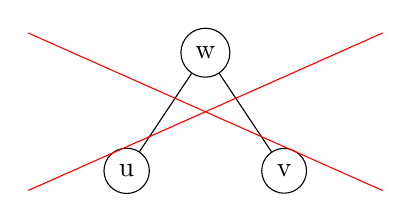
\begin{tikzpicture}[level/.style={sibling distance = 2cm/#1,
			level distance = 1.5cm},
		every node/.style = {shape=circle, draw, align=center}]
		\node{w}
			child {node{u}}
			child {node{v}};
		\draw[red] (-2.25,0.25)--(2.25,-1.75);
		\draw[red] (2.25,0.25)--(-2.25,-1.75);	
		\end{tikzpicture}
		\caption{Widerspruch}
	\end{subfigure}
	\begin{subfigure}{0.24\textwidth}
		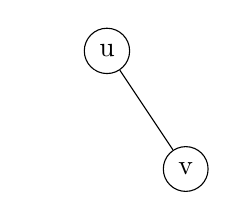
\begin{tikzpicture}[level/.style={sibling distance = 2cm/#1,
			level distance = 1.5cm},
		every node/.style = {shape=circle, draw, align=center}]
		\node{u}
		child[white] {}
		child {node{v}};	
		\end{tikzpicture}
		\caption{Variante 1}
	\end{subfigure}
	\begin{subfigure}{0.24\textwidth}
		\begin{tikzpicture}[level/.style={sibling distance = 3cm/#1,
			level distance = 1.5cm},
		every node/.style = {shape=circle, draw, align=center}]
		\node{v}
		child {
			node{u}
		}
		child[white] {};	
		\end{tikzpicture}
		\caption{Variante 2}
	\end{subfigure}
	\begin{subfigure}{0.24\textwidth}
		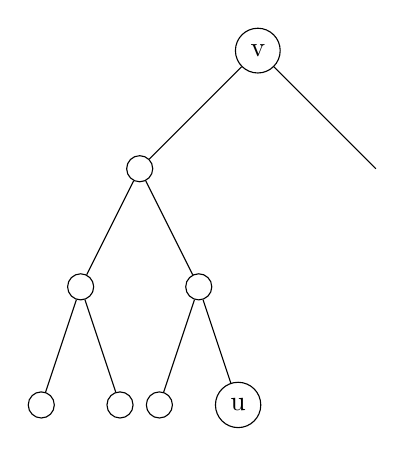
\begin{tikzpicture}[level/.style={sibling distance = 3cm/#1,
			level distance = 1.5cm},
		every node/.style = {shape=circle, draw, align=center}]
		\node{v}
		child {
			node{}
			child{
				node{}
				child{node{}}
				child{node{}}
			}
			child{
				node{}
				child{node{}}
				child{node{u}}
			}
		}
		child {};	
		\end{tikzpicture}
		\caption{Variante 3}
	\end{subfigure}
\end{figure}
Angenommen es gäbe einen LCA(u,v) w ungleich u oder v, so ist w "`zwischen"' u und v im Widerspruch zur Annahme, dass v unmittelbarer Nachfolger von u ist. Somit gilt, dass w gleich u oder v ist.\qed
\subsection{b)}
\paragraph{Fall 1}
Offensichtlich gilt $\Delta(T)=\delta(v_{2^h-2},v_{2^h-1}) = h$, wobei $v_{2^h-2}$ das letzte Element der Traversierung des linken Teilbaumes ist (vergleiche u aus Abb d)) und $v_{2^h-1}$ die Wurzel ist (vergleiche v aus Abb d)).
\paragraph{Fall 2}
$\Delta(T)=1$, da $\delta(v_i,v_{i+1}) = 1 ~\forall i \in ( 0,\ldots,h-1 )$
\section{Aufgabe 2}
\subsection{a)}
Angenommen es gäbe einen MST $\tilde{T}$ von G und eine lokal minimale Kante $(u,v)$ in G aber nicht in $\tilde{T}$. Das $\tilde{T}$ MST gilt es existiert ein Pfad von $u$ nach $v$ in $\tilde{T}$. Da $(u,v)$ lokal minimal ist gilt auch, $\delta((u,v)) < \delta((u,w))$ mit $(u,w)$ in $\tilde{T}$ und $w\neq v$. Nun gilt offensichtlich:
\begin{enumerate}
	\item Durch das entfernen von $(u,w)$ und hinzunehmen von $(u,v)$ sinkt das gesamt Gewicht
	\item Durch das entfernen von $(u,w)$ und hinzunehmen von $(u,v)$ entsteht wieder ein Baum
\end{enumerate}
Somit gilt der neue Baum $T$ ist kleiner als $\tilde{T}$ im Widerspruch zur Annahme $\tilde{T}$ sei MST.\\
$\Rightarrow$ Jede lokal minimale Kante gehört zu allen MST in G.\qed
\subsection{b)}
\paragraph{zu zeigen}
Die Menge aller lokal minimalen Kanten eines Graphen ist ein Wald $\Rightarrow$ Es reicht zu zeigen: Die Menge aller minimalen Kanten eines Graphen ist zykelfrei
\paragraph{Beweis}
Angenommen es existiert ein Zyklus. Dank der injektiven Gewichtsfunktion existiert genau eine Kante $(u,v)$ mit maximalem Gewicht in diesem Zyklus. Da es sich um einen Zyklus handelt, existieren die Kanten $(u,t)$ und $(v,w)$. Da $(u,v)$ maximales Gewicht im Zyklus hat gilt: \[ \delta((u,t)) < \delta((u,v)) > \delta((v,w)) \]
$\Rightarrow$ $(u,v)$ ist nicht minimal im Widerspruch zur Annahme.\qed
\section{Aufgabe 3}
\subsection{Bor\r{u}vka in $O(|E|\log|V|)$}
Wir initialisieren unseren Wald $F$ mit $(V,\emptyset)$. In jeder Iteration, sucht jeder Baum $T$ in $F$ die leichteste Kante in $G$, die $T$ verlässt und markiert diese. Anschließend werden alle markierten Kanten $F$ hinzugefügt und wieder demarkiert. Dies wird wiederholt, bis $F$ komplett verbunden ist. Wie im letzten Blatt gezeigt, folgt eine Laufzeit in $O(|E|\log|V|)$.
\subsection{Bor\r{u}vka in $O(|V|^2)$}
Wir starten mit unserem Graphen $G_0=(V_0,E_0)$. In jeder Iteration $i$ initialisieren wir einen Wald $F_i$ mit $(V_i,\emptyset)$. Jeder Knoten $v\in V_i$ in $F_i$ sucht die leichteste Kante in $G_i$, die $v$ verlässt un markiert diese. Anschließend werden alle markierten Kanten $F_i$ hinzugefügt. Nun wird $G_i$ mit den in $F_i$ gewählten Kanten reduziert, also alle in $F_i$ verbunden Knoten werden zu einem Überknoten zusammengefasst. $G_{i+1}$ ist nun der Graph, der aus der so zusammengefassten Knotenmenge $V_{i+1}$ besteht und allen angepassten Kanten, ohne 1- und 2-Zykel-Kanten ( z.B. $(u,u)$ oder $(u,v),(v,u)$ ). Mit der gleichen Argumentation wie im letzten Blatt kann man sagen, dass $|V_{i+1}| \in O\left(\frac{|V_i|}{2}\right)$ gilt. Der Algorithmus terminiert, wenn $|V_i| = 1$. Die Lösung sind dann alle bislang hinzugefügt Kanten. Wenn wir $|E_i| \leq |V_i|^2$ abschätzen folgt für eine Iteration eine Laufzeit von $O(|V_i|^2)$. Somit gilt, dass die Laufzeit in $O\left( |V|^2 + \left(\frac{|V|}{2}\right)^2 + \left(\frac{|V|}{4}\right)^2+\ldots \right) = O(|V|^2)$
\subsection{Bor\r{u}vka in $O\left(|E|\log\left(\frac{|V|^2}{|E|}\right)\right)$}
Wir nehmen beide Algorithmen und nutzen in jeder Iteration den gerade schnelleren, damit erhalten wir pro Iteration eine Laufzeit von $O(|E_i|)$ wobei $|E_i|$ durch $|E|$ und $|V_i|^2$ begrenzt ist. Wir wählen also den 1. Algorithmus solange gilt $|E| < |V_i|^2$. Dies passiert in der $j = \frac{1}{2}\log\left(\frac{|V|^2}{|E|}\right)$ Iteration, da gilt:
\begin{align*}
				&|E| = |V_i|^2\\
\Leftrightarrow &|E| = \left(\frac{|V|}{2^i}\right)^2 = \frac{|V|^2}{2^{2i}}\\
\Leftrightarrow &2^{2i} = \frac{|V|^2}{|E|}\\
\Leftrightarrow &2i = \log_2\left(\frac{|V|^2}{|E|}\right)\\
\Leftrightarrow &i = \frac{1}{2}\log_2\left(\frac{|V|^2}{|E|}\right)
\end{align*}
Die ersten $j$ Iterationen je $O(|E|)$ lange und für die restlichen insgesamt $O\left(\sum_{i\geq j}^{|V_i|^2}\right)$ $|V_j|^2$ war gerade $|E|$ und somit gilt 
\[O\left( |V_j|^2 + \left(\frac{|V_j|}{2}\right)^2 + \left(\frac{|V_j|}{4}\right)^2+\ldots \right) = O\left( |E| + \frac{|E|}{4} + \frac{|E|}{16}+\ldots \right) = O(|E|)\]
Daraus folgt eine gesamt Laufzeit für den Algorithmus von $O(|E|(1+j)) = O\left( |E| + |E|\frac{1}{2}\log\left(\frac{|V|^2}{|E|}\right) \right) =  O\left( |E|\frac{1}{2}\log\left(\frac{|V|^2}{|E|}\right) \right)$\\
Der Algorithmus arbeitet Korrekt, da er das Ergebnis der beiden anderen Algorithmen nicht verändert.
\end{document}